\section{Verfahren zur Ausreißererkennung}
Verfahren zur Ausreißererkennung bewerten die übergebenen Daten mithilfe eines Ausreißer"=Scores, der ihre Wahrscheinlichkeit bewertet, ein Ausreißer zu sein. Die Verfahren in den ersten zwei Abschnitten können von diesem Score allerdings nicht direkt ableiten, ob ein Datenpunkt ein Ausreißer ist oder nicht, sondern sie geben einen festgelegten Prozentsatz der Datenpunkte zurück, die am schlechtesten abschneiden. Im dritten und letzten Abschnitt wird dann ein Verfahren präsentiert, das selbst einen Schwellwert festlegt, ab dem es einen Punkt als Ausreißer markiert, was auch dazu führen kann, dass keine Ausreißer gefunden werden, im Gegensatz zu den ersten beiden Verfahren.

\subsection{k"=Nearest"=Neighbors}
Das k"=Nearest"=Neighbors- oder knn"=Verfahren zur Ausreißererkennung von Sridhar Ramaswamy et al. \cite{knn} erkennt Ausreißer dadurch, dass sie eine größere Distanz zu anderen Punkten besitzen. Um die Distanz zu berechnen, wird in der verwendeten Bibliothek PyOD \cite{pyod} die Minkowski"=Distanz \cite{minkowski} benutzt, die zwischen zwei Punkten $x = (x_0,x_1,\ldots,x_{n-1})$ und $y=(y_0,y_1,\ldots,y_{n-1})$ die Distanz $d(x,y)$ wie folgt berechnet:
\[d(x,y) = \left(\sum_{i=0}^{n-1}|x_i - y_i|^p\right)^{\frac{1}{p}}.\]
Der Parameter $p$ wird von PyOD standardmäßig auf 2 gesetzt, wodurch wir einen Spezialfall der Minkowski"=Distanz erhalten, und zwar die Euklidische Distanz, die auch beim Maß der Ähnlichkeit in \autoref{subsec:aehnlichkeit} benutzt wird. Was knn nun macht ist, dass es von allen Punkten die Abstände zu allen anderen Punkten berechnet und für den jeweiligen Punkt speichert. Daraufhin merkt es sich nur die $k$ Stück, die am nächsten sind, und setzt den Ausreißer"=Score auf die Distanz des am weitesten entfernten Punkts, unter diesen $k$ Stück. Punkte mit einem hohen Ausreißer"=Score haben weniger Punkte, die dicht an ihnen dran sind, und sind somit offensichtlich Ausreißer. PyOD setzt außerdem standardmäßig den Wert $k=5$. Upmanu Lall und Ashish Sharma \cite{kauswahl} sowie Shichao Zhang et al. \cite{kauswahl2} nutzen ebenfalls diesen Wert, versuchen allerdings möglichst effizient ein optimales $k$ für einen gegebenen Datensatz zu finden. Da $k=5$ de facto ein etablierter Standardwert ist und genauere Analysen über die Auswirkungen des Parameters umfangreich \cite{kauswahl2} und nicht zentral für diese Arbeit sind, da es nicht um die Optimierung des Algorithmus, sondern um die Auswirkungen der Kompression geht, wird er in der Implementierung nicht geändert.

\subsection{Isolation Forest}
Das Isolation"=Forest- oder iForest"=Verfahren zur Ausreißererkennung von Fei Tony Liu et al. \cite{iForest} erkennt Ausreißer dadurch, dass sie leichter von anderen zu isolieren sind. Isolieren bedeutet hierbei das Abgrenzen eines Punktes von anderen. Ausreißer sind leichter abzugrenzen, da sie zwei Eigenschaften besitzen:
\begin{enumerate}
    \item "`Ausreißer sind eine Minderheit, die aus wenigen [Datenpunkten] besteht"',
    \item "`Sie besitzen Werte, die sich stark von denen normaler [Datenpunkte] unterscheiden"'.
\end{enumerate}
(vergleiche \cite[Ch. 1]{iForest}, aus dem Englischen übersetzt) \\
iForest isoliert Datenpunkte, indem es sie so lange zufällig rekursiv partitioniert, bis nur noch ein Datenpunkt in einer Partition liegt. Diese zufällige Partitionierung sorgt dafür, dass Ausreißer mit nur wenigen Partitionen isoliert werden, da es nur wenige Datenpunkte sind, die sich von den anderen stark unterscheiden. Um diese Idee visuell zu verdeutlichen, veranschaulicht die \autoref{fig:partitionierungen} eine Isolierung von einem normalen Datenpunkt $x_i$ und von einem Ausreißer $x_0$. Dabei sind die kleinen Kreise die verschiedenen Datenpunkte und die schwarzen Linien die Grenzen der Partitionen. In \autoref{subfig:partitionierung1} sieht man nun, dass zur Isolierung von $x_i$ viele zufällige Partitionen benötigt werden. In \autoref{subfig:partitionierung2} sieht man wiederum, dass $x_0$ relativ schnell, mit nur zwei zufälligen Partitionen, isoliert werden konnte.
\begin{figure}[bth]
  \subfloat[Isolierung von $x_i$]{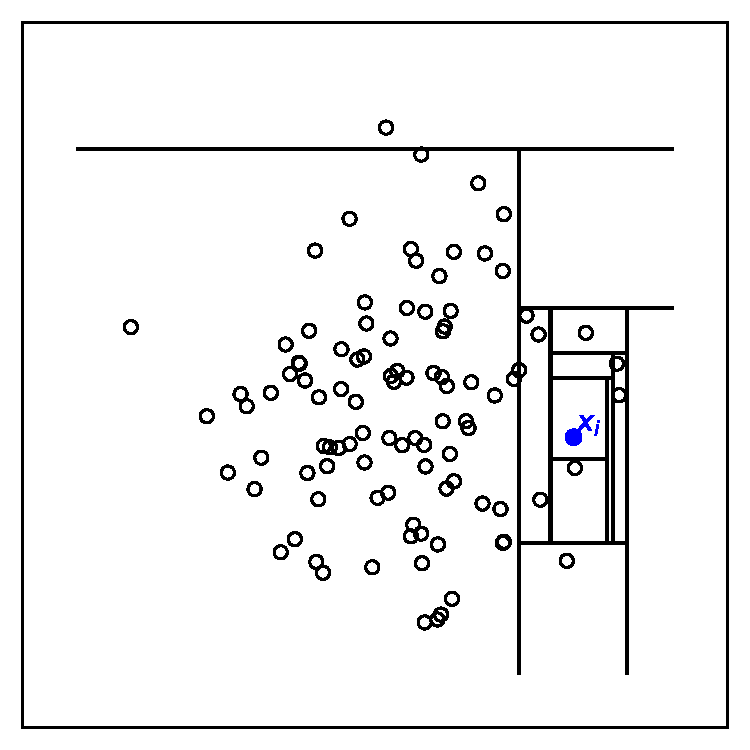
\includegraphics[width=0.49\textwidth]{Graphics/Partitionierung1.pdf}\label{subfig:partitionierung1}}\hfill
  \subfloat[Isolierung von $x_0$]{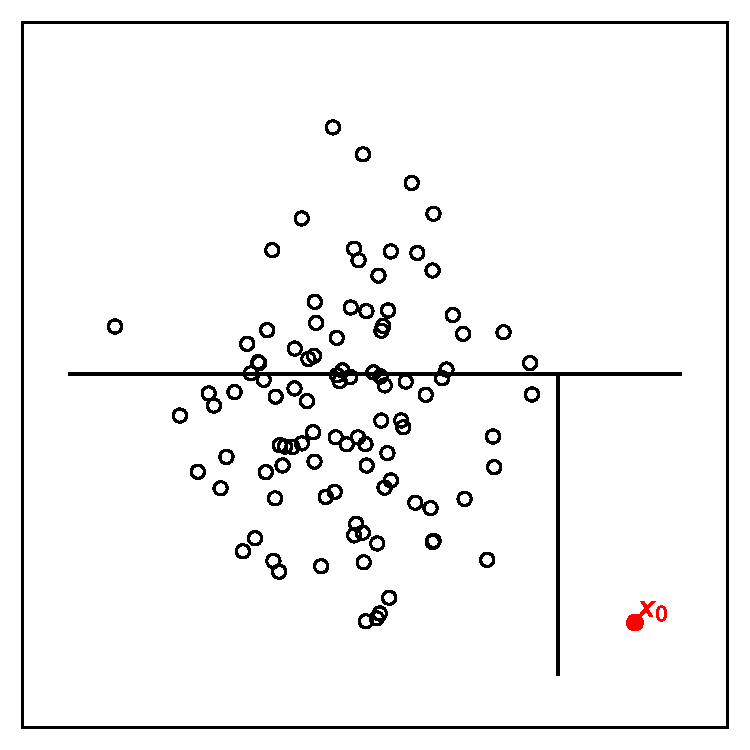
\includegraphics[width=0.49\textwidth]{Graphics/Partitionierung2.pdf}\label{subfig:partitionierung2}}\hfill
  \caption{Zufällige Partitionierung zur Isolierung zweier Punkte, angelehnt an \cite[Fig. 1]{iForest}}
  \label{fig:partitionierungen}
\end{figure}

Das rekursive Partitionieren lässt sich auch als Baum darstellen, wobei dann die Pfadlänge von der Wurzel zu einem Knoten genau der Anzahl der Partitionen entspricht. Daher kommt auch der Name iForest, da mehrere dieser Bäume zur Isolierung generiert werden, um, durch die zufällige Partitionierung, Partitionen mit verschiedenen Daten zu erhalten. Die durchschnittliche Pfadlänge der verschiedenen Datenpunkte ist dann die erwartete Pfadlänge. Die Baumstruktur baut sich wie folgt auf: Zuerst wird aus der Beobachtung in $ZR$ eine zufällige Teilmenge $X$ ausgesucht, meist nicht mehr als 256 Elemente, da dies zu genaueren Ergebnissen führt \cite[Ch. 4.1]{iForest}. Dann beginnt die Konstruktion des Baums, indem die Menge $X$ in die Wurzel des Baums geschrieben wird. Daraufhin wird ein zufälliges Feature ausgesucht und ein zufälliger Wert $p$, der zwischen dem Minimum und Maximum von diesem Feature liegt. Die Menge $X$ wird dann, dem Wert $p$ entsprechend, in zwei disjunkte Teilmengen aufgeteilt, wobei die kleineren Werte in den linken Kindknoten und die größeren Werte in den rechten Kindknoten der Wurzel geschrieben werden. Die Schritte ab der Auswahl des zufälligen Features werden nun für die Kindknoten so lange fortgeführt, bis entweder:
\begin{itemize}
    \item "`der Baum eine maximale Höhe erreicht hat"',
    \item "`$|X|=1$"' oder
    \item beim zufällig ausgewählten Feature "`alle Werte der Elemente in $X$  identisch sind"'.
\end{itemize}
(vergleiche \cite[Ch. 2]{iForest}, aus dem Englischen übersetzt) \\
Etwa 100 Bäume genügen \cite[Ch. 4.1]{iForest}, um keine signifikanten Unterschiede mehr in der durchschnittlichen Pfadlänge zwischen Wurzel und einem Knoten zu erhalten. Um dann einen Ausreißer"=Score $s$ in Abhängigkeit vom Knoten $x$ und der Anzahl $n = |X|$ zu erhalten, wird folgende Formel angewandt:
\[ s(x,n)=2^{-\frac{E(h(x))}{c(n)}} ,\quad c(n) = 2 H(n-1) - \frac{2(n-1)}{n} ,\quad H(i) = \ln(i) + \gamma \]
mit der Euler"=Mascheroni"=Konstante $\gamma=0{,}5772156649$. Weiter sind $h(x)$ die Pfadlänge eines Knotens $x$ in einem Baum, also die Kantenanzahl von der Wurzel bis zu diesem Knoten, und $E(h(x))$ die durchschnittliche Kantenanzahl über alle Bäume. Diese Formel normalisiert die durchschnittliche Höhe und garantiert damit, dass wir immer $0 < s \le 1$ erhalten, egal für welches $n$ und $x$. Mit $s$ kann man nun drei Einschätzungen vornehmen:
\begin{itemize}
    \item "`ist das $s$ eines Knoten nah an 1, dann ist er definitiv ein Ausreißer"',
    \item "`ist das $s$ eines Knoten weit unter 0,5, dann kann man mit Sicherheit sagen, dass er ein normaler [Datenpunkt] ist"',
    \item "`geben alle [Datenpunkte] $s \approx 0{,}5$ zurück, dann gibt es keine auffälligen Ausreißer"'.
\end{itemize}
(vergleiche \cite[Ch. 2]{iForest}, aus dem Englischen übersetzt)

\subsection{Random Projections mit Median"=Absolute"=Deviation}
Dieses Verfahren orientiert sich stark an dem von Paula Navarro-Esteban und Juan Antonio Cuesta-Albertos \cite{randomProjection}. Es beruht auf der Idee, dass man multivariate Daten auf mehrere eindimensionale Werte projiziert und je Projektion eine univariate Ausreißererkennung anwendet. Projektion bedeutet hierbei, dass das Skalarprodukt zwischen zwei Vektoren berechnet wird. In unserem Kontext wird also das Skalarprodukt zwischen dem Vektor $x$ mit den Werten einer Zeitreihe und einem Vektor $y$ mit zufälligen, positiven Werten gebildet. Das Skalarprodukt entspricht der Summenformel $\sum_{i=0}^{n-1} x_iy_i$, wobei $n$ die Anzahl der Komponenten der Vektoren ist, beziehungsweise die Länge der Zeitreihe. Der Grund dieser Projektion ist, dass Zeitreihen, die ähnliche Werte haben, auch ähnliche Projektionswerte besitzen, Zeitreihen, die sich komplett anders verhalten, haben wiederum stark abweichende Projektionswerte. 

Was das Verfahren also nun macht ist, dass es einen Vektor mit zufälligen, positiven Werten erstellt und diesen mit allen Zeitreihen verknüpft, um eine Liste an Projektionswerten zu erhalten. Auf diese Liste wird dann, wie in \cite[Ch. 3.3]{randomProjection}, das univariate Ausreißererkennungs"=Verfahren Median"=Absolute"=Deviation angewendet. Diese Erstellung eines zufälligen Vektors, mit anschließender Projektion und Ausreißererkennung, wird jetzt 50 Mal wiederholt, da dies ein Wert ist, der für keinen hohen Rechenaufwand sorgt und gleichzeitig ausreichend hoch ist, um die Zufallseffekte einzelner Projektionen zu glätten und stabile, reproduzierbare Ergebnisse bei der Ausreißererkennung zu gewährleisten \cite[Ch. 4.1]{randomProjection}. In einer separaten Liste wird gespeichert, wie oft eine Zeitreihe als Ausreißer erkannt wurde. Diese Liste wird wieder mithilfe von Median"=Absolute"=Deviation auf Ausreißer untersucht, damit Zeitreihen, die z.~B. nur ein einziges Mal als Ausreißer erkannt wurden und damit wahrscheinlich kein echter Ausreißer sind, nicht als Ausreißer zurückgegeben werden.

Median"=Absolute"=Deviation ist ein simples Verfahren, um auf univariaten Daten Ausreißer zu erkennen \cite[Ch. 3.3]{mad}. Für die univariaten Daten $X=[x_0,x_1,\ldots, x_{n-1}]$ wird zuerst der Median berechnet: \[\Median(X)=\left\{ \begin{array}{ll}
    x_{\frac{n-1}{2}} & \text{falls } n \text{ ungerade} \\
    0{,}5 (x_{\frac{n}{2}-1} + x_{\frac{n}{2}}) & \text{falls } n \text{ gerade} \\
\end{array} \right..\]
Dann wird der Median der absoluten Abweichungen um den Median der Daten (MAD) berechnet, das heißt für jedes Element $x_i$ in $X$ wird die Differenz $|x_i - \Median(X)|$ berechnet, und der Median der Menge dieser Differenzen ist der MAD"=Wert. Nun wird ein Schwellwert $d$ festgelegt, der multipliziert mit dem MAD"=Wert den Bereich um den Median der Daten festlegt, in dem keine Ausreißer liegen. Das heißt ein Wert $x_i$, der $\Median(X) - d \cdot \text{MAD} < x_i < \Median(X) + d \cdot \text{MAD}$ erfüllt, ist ein normaler Wert, wenn nicht, ist es ein Ausreißer. Boris Iglewicz und David C. Hoaglin \cite[Ch. 3.3]{mad} empfehlen auf Grundlage ihrer eigenen Studie einen Schwellwert von $d=3{,}5$, während Christoph Leys et al. \cite[p. 766]{mad2} Schwellwerte von 3, 2,5 und 2 vorschlägt, in einem darauffolgenden Abschnitt aber auch feststellt, dass in seinem Beispiel etwa 3,5 ein optimaler Wert ist.
